\subsection*{Exercise 2 solution}

Here follows the listing for the \emph{header file} that contains all the
declarations of the functions in the code.
% zerofun.hpp
\lstset{basicstyle=\scriptsize\sf}
    \lstinputlisting[caption=Function declarations for computing the zero of a
    function.] {src/zerofun.hpp}
\lstset{basicstyle=\sf}

We put the corresponding definitions in the \emph{source file}
\texttt{zerofun.cpp}:
\lstset{basicstyle=\scriptsize\sf}
    \lstinputlisting[caption=Function definitions for computing the zero of a
    function.] {src/zerofun.cpp}
\lstset{basicstyle=\sf}

The instruction \texttt{assert(u*f(b)<0.0);} is used to perform a simple error
checking. If the boolean instruction inside is not verified, the program stop
immediately and an error message is generated.

We have also the listing for the file \texttt{bn.cpp} that contains the main
program
\lstset{basicstyle=\scriptsize\sf}
    \lstinputlisting[caption=function definition and main program.]
    {src/bn.cpp}
\lstset{basicstyle=\sf}

The compilation can be peformed with
\begin{verbatim}
g++  -c -o bn.o bn.cpp -Wall
g++  -c -o zerofun.o zerofun.cpp -Wall
g++  -o bn bn.o zerofun.o
\end{verbatim}

The files \texttt{bn.o} and \texttt{zerofun.o} are the translation to object
code of the type and function definitions that we wrote in the corresponding
source files. The executable \texttt{bn} is created throught the \emph{linking}
of the object files together with the necessary libraries.

The \cpp{assert} can be disabled with the \cpp{-DNDEBUG} flag that must be
passed to the compiler when compiling files that contain it, i.e.
\begin{verbatim}
g++  -c -o bn.o bn.cpp -Wall
g++  -c -o zerofun.o zerofun.cpp -Wall -DNDEBUG
g++  -o bn bn.o zerofun.o
\end{verbatim}

In order to graphically see the error, it is possible to pass two additional
arguments to the functions  \texttt{bisection}, \texttt{newton} and
\texttt{robust}. The first one is the exact solution, while the second is the
name of the file for the output.
The listing for the \texttt{bng.cpp} file is as follows
\lstset{basicstyle=\scriptsize\sf}
    \lstinputlisting[caption=Function definition and main program.]
        {src/withGnuplot/bng.cpp}
\lstset{basicstyle=\sf}

we note at the end the call to the operating system that uses the file
\texttt{print\_data} with the following commands
\begin{verbatim}
set terminal png
set output "graph.png"
plot "data" with lines
\end{verbatim}
The listing for \texttt{zerofung.hpp} is basically the same as
\texttt{zerofun.hpp}, while the listing for \texttt{zerofung.cpp} is
\lstset{basicstyle=\scriptsize\sf}
    \lstinputlisting[caption=Definitions for the functions to compute a zero of
        a function.]{src/withGnuplot/zerofung.cpp}
\lstset{basicstyle=\sf}

Note how the functions \texttt{bisection} and \texttt{newton} manage the file.
First of all it is declared, using the scope resolution operator \cpp{::} to
access the members in the \cpp{std} namespace. Afterwards it is opened in the
out mode for \texttt{bisection}, and out and app for \texttt{newton}.i This
means that in the second case the files are written at the end of the file,
without deleting any previous content. There is also a test to verify that the
file has been properly opened. The data output is performed inside the loops in
a way that is totally similar to printing to screen. at the end of each function
the file is closed.

This is the graph generated by the code
\begin{figure}[!h]
    \centering
    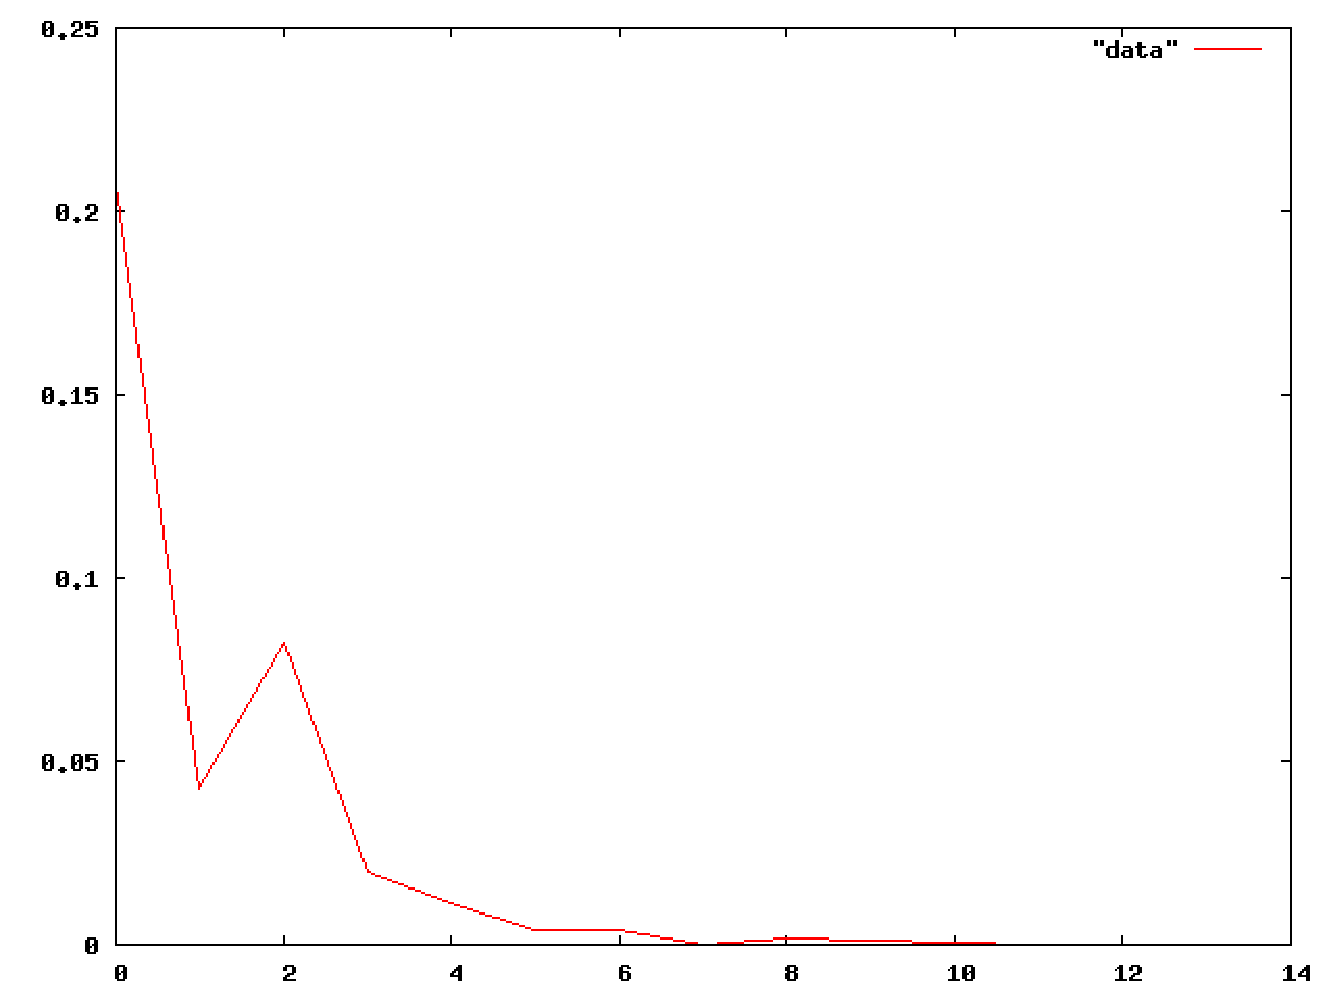
\includegraphics[width=0.7\textwidth]{./images/graph}
\end{figure}
